\documentclass[conference]{IEEEtran}
\IEEEoverridecommandlockouts
% The preceding line is only needed to identify funding in the first footnote. If that is unneeded, please comment it out.
\usepackage{cite}
\usepackage{amsmath,amssymb,amsfonts}
\usepackage{algorithmic}
\usepackage{graphicx}
\usepackage{textcomp}
\usepackage{xcolor}
\usepackage{booktabs}
\usepackage{subfigure}
\def\BibTeX{{\rm B\kern-.05em{\sc i\kern-.025em b}\kern-.08em
    T\kern-.1667em\lower.7ex\hbox{E}\kern-.125emX}}
\usepackage{listings}
\usepackage[utf8]{inputenc}


% Default fixed font does not support bold face
\DeclareFixedFont{\ttb}{T1}{txtt}{bx}{n}{8} % for bold
\DeclareFixedFont{\ttm}{T1}{txtt}{m}{n}{8}  % for normal

% Custom colors
\usepackage{color}
\definecolor{deepblue}{rgb}{0,0,0.5}
\definecolor{deepred}{rgb}{0.6,0,0}
\definecolor{deepgreen}{rgb}{0,0.5,0}

\usepackage{listings}

% Python style for highlighting
\newcommand\pythonstyle{\lstset{
language=Python,
basicstyle=\ttm,
otherkeywords={self,add},             % Add keywords here
keywordstyle=\ttb\color{deepblue},
emph={zynet,__init__},          % Custom highlighting
emphstyle=\ttb\color{deepred},    % Custom highlighting style
stringstyle=\color{deepgreen},
frame=tb,                         % Any extra options here
showstringspaces=false            % 
}}


% Python environment
\lstnewenvironment{python}[1][]
{
\pythonstyle
\lstset{#1}
}
{}

% Python for external files
\newcommand\pythonexternal[2][]{{
\pythonstyle
\lstinputlisting[#1]{#2}}}

% Python for inline
\newcommand\pythoninline[1]{{\pythonstyle\lstinline!#1!}}


\begin{document}

\title{ZyNet: Automating Deep Neural Network Implementation on Low-cost Reconfigurable Edge Computing Platforms}

\maketitle

\begin{abstract}
Prevalence of internet of things (IoT) enabled applications provide a new opportunity to low-cost FPGA devices to act as edge computing nodes. Although FPGA vendors provide development environment for FPGA-based neural networks, they often support only high-end FPGAs. At the same time these platforms are not as user friendly as their software counter parts. In this work we introduce ZyNet, a Python package, which enables faster implementation of deep neural networks targeting low-cost hybrid FPGA platforms such as the Xilinx Zynq. Based on hardware-software co-design philosophy this platform supports pre-trained or on-board trained networks with development environment very similar to the popular TensorFlow environment. Implementation results show that the platform achieves accuracy very close to software implementations at the same time gives performance improvement of several orders compared to other edge computing devices. The platform is integrated with Xilinx development tools and is distributed as open source through the Python Package Index (PyPI) and git repositories. 
\end{abstract}

\begin{IEEEkeywords}
neural networks, hardware-software co-design, edge computing
\end{IEEEkeywords}

\section{Introduction}
\label{sec:intro}

Advent of IoT-enabled applications have stimulated the interest for neural networks on edge computing devices.
These are low-cost devices with limited computing and memory capabilities and require a low energy footprint.
It has been shown many a times that FPGAs can outperform software implementation of deep neural network~(DNN) as their architecture is friendly to the concurrent architecture of neural networks~\cite{Huimin2016}.
Although FPGA-based DNNs have found their way to datacenters, they are still not popular for edge computing due to their power consumption and limited flexibility.
Hybrid FPGA platforms such as Xilinx Zynq devices are promising in this regard as they are relatively cheaper, low power consuming and can support a hardware-software co-design approach for better flexibility.

Another stumbling block for FPGA-based neural computing is the lack of programmer friendly development environment.
Although FPGA vendors are providing AI/ML platforms~\cite{xilinxddnk}, they often require high-end devices for implementation and tool flow are challenging to follow.
In this work we introduce ZyNet, a Python package which not only generates synthesizable DNN code, but automatically integrates it with necessary peripherals to provide a complete system solution.
The target implementation platforms are low-cost hybrid FPGA platforms such as ZedBoard and MicroZed, but the solution can be equally extended to any other FPGA platform.
The generated DNN RTL code are vendor agnostic and can be implemented with any logic synthesize tool.

The remainder of this paper is organized as as the following, Section~\ref{sec_background} discusses the motivation and background, Section~\ref{sec_architecture} discusses the architecture of ZyNet, Section~\ref{sec_results} discusses the implementation results and Section~\ref{sec_conclusion} concludes the paper and recommends future research directions.
\section{Motivation and Background}
\label{sec_background}

The code snippet below shows the implementation of a 5-layer DNN in TensorFlow with 4 hidden layers with 30, 30, 10 and 10 neurons each.
Each layer uses ReLU-based activation function and an output \emph{softmax} layer is used to determine the output neuron with maximum value. 
The programing model is very intuitive, flexible, scalable and programmer friendly. 

\begin{python}
import tensorflow as tf
model = tf.keras.models.Sequential()
model.add(tf.keras.layers.Flatten())
model.add(tf.keras.layers.Dense(30,activation=tf.nn.relu))
model.add(tf.keras.layers.Dense(30,activation=tf.nn.relu))
model.add(tf.keras.layers.Dense(10,activation=tf.nn.relu))
model.add(tf.keras.layers.Dense(10,activation=tf.nn.relu))
model.add(tf.keras.layers.Dense(10,activation=tf.nn.softmax))
model.compile(optimizer='adam',metrics=['accuracy'],
loss='sparse_categorical_crossentropy')
\end{python}

Our aim is to develop a model, which is similar to TensorFlow but generates efficient hardware tageting FPGAs.
The snippet below describes the same network as before, but generates Verilog RTL code, which can be synthesized and implemented using any target FPGA vendor tools.
Since hardware implementation provides bit-level precision of data width, three additional parameters are provided with the \emph{compile} method. 

\begin{python}
import zynet as zn
model = zn.zynet.model()
model.add(zn.zynet.layer("flatten",784))
model.add(zn.zynet.layer("Dense",30,"relu"))
model.add(zn.zynet.layer("Dense",30,"relu"))
model.add(zn.zynet.layer("Dense",10,"relu"))
model.add(zn.zynet.layer("Dense",10,"relu"))
model.add(zn.zynet.layer("Dense",10,"hardmax"))
model.compile(pretrained='No',dataWidth=16,
    weightIntSize=4,inputIntSize=1)
\end{python}

The \emph{dataWidth} specifies total bit width of input data, bias and weight values. \emph{InputIntSize} and \emph{weightIntSize} specifies the number of bits used to represent the integer portion of input and weight values.
Since ZyNet implementations use fixed point representation, these parameters are required for internal calculations.
For \emph{pretrained} networks, where weight and bias values are available before network synthesis, these parameters can be automatically determined by the tool by analyzing the maximum and minimum values.
\section{Architecture}
The following section discusses the architecture of the deep neural network generated by ZyNet, its parameters and application interface.
\subsection{Neuron}
\begin{figure}[!t]
\centering
   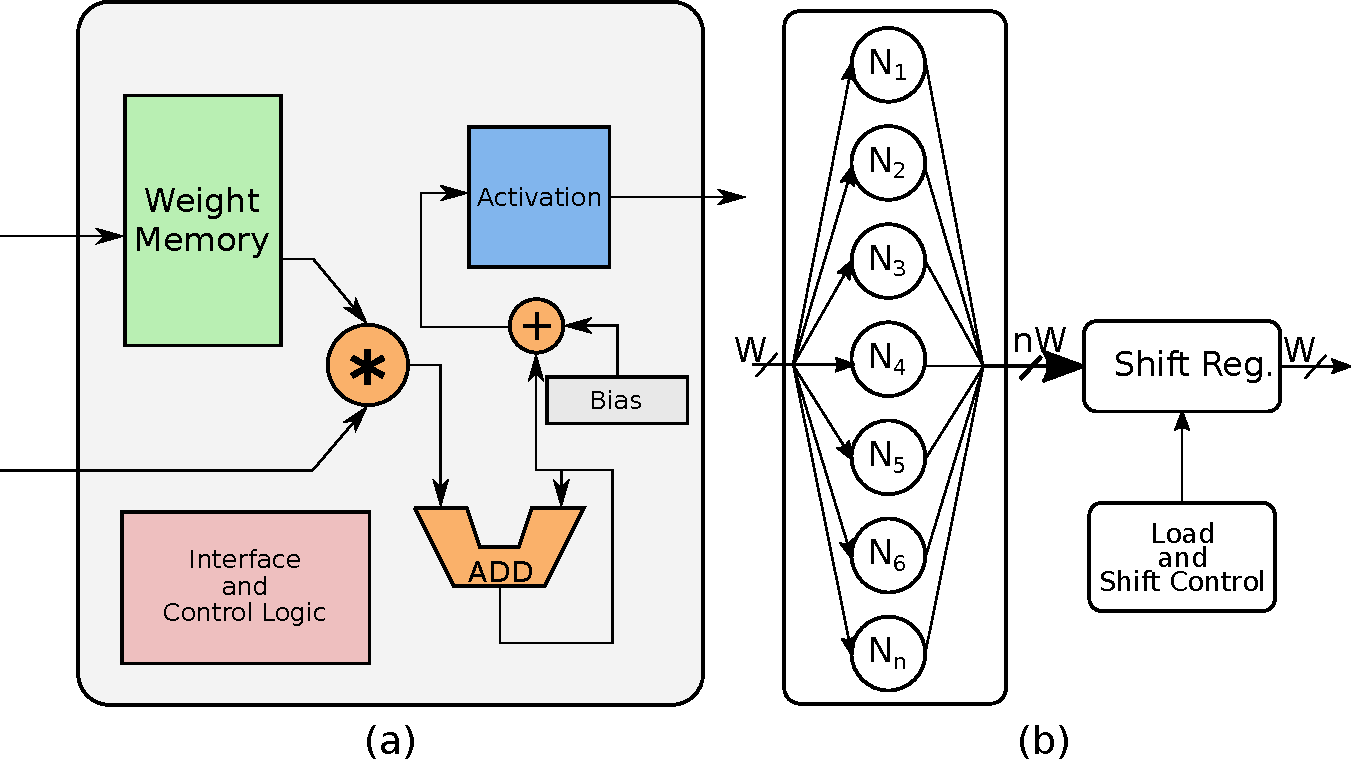
\includegraphics[width=\columnwidth]{Figures/neuron.pdf}
   \caption{Neuron Architecture}
   \label{fig:neuron}
   \vspace{-3mm}
\end{figure}
The architecture of a single artificial neuron is as shown in Fig.~\ref{fig:neuron}.
Each neuron has independent interfaces for configuration (weight, bias etc.) and for streaming data in and out.
Irrespective of number of neighbors, each neuron has a single interface for accepting data.
This enables scalability of the network and improves clock performance by compromising on latency. 

An internal memory, whose size is decided by the number of inputs to the neuron, is used to store the weight values corresponding to each input.
Depending on whether the network is configured as \emph{pre-trained} or not, either a RAM with read and write interface or a ROM initialized with weight values are instantiated.
As inputs are streamed into the neuron, a control logic reads the corresponding weight value from the memory.
Inputs and corresponding weight values are multiplied and accumulated (MAC) and finally added with the \emph{bias} value.
Like the weights, the bias value is stored in a register at implementation time if the network is \emph{pre-trained} or configured at run-time with software.
The output from the MAC unit is finally applied to the activation unit.
Based on the type of activation function configured (Sigmoid, ReLU, hardMax etc.), either a look-up-table based (for Sigmoid) or a circuit-based function is implemented by the tool.
The type of function chosen has a direct impact on the accuracy of the network and the total resource utilization and clock performance. 

\subsection{Layer}
Each layer instantiates user specified number of neurons and manages data movement between the layers.
Since each neuron has a single data interface and a fully connected layer requires connection to every neuron in the previous layer, data from each layer is initially stored in a shift register.
It is then shifted to the next layer one per clock cycle.

\subsection{System Architecture}
Fig.~\ref{fig:sysarch} depicts the complete system architecture generated by ZyNet when targeting the Zynq platform.
It packages ZyNet as an IP core and automatically integrates with other peripherals.
The AXI4-Lite interface of ZyNet is connected to the GP0~(General Purpose) interface of Zynq PS~(processing system).
This interface is used for configuration in case of untrained networks and for reading out the final network output in case of both pre-trained and untrained network.

The streaming interface from ZyNet is connected to a DMA controller, which in turn is connected to the external memory through the Zynq HP0 (high performance) interface.
This enables training and test data to be directly streamed from external memory to ZyNet.
The DMA controller is also interfaced with the Zynq GP port for configuration.
Interrupt signals from both ZyNet and DMA controller are connected to the PS interrupt interface.
 
\begin{figure}[!t]
\centering
   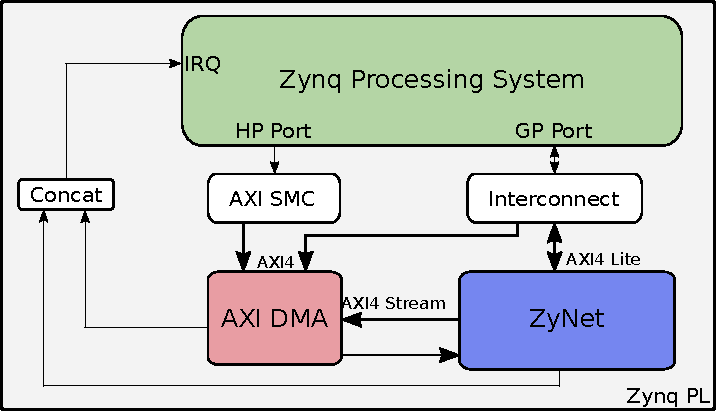
\includegraphics[width=0.8\columnwidth]{Figures/arch.pdf}
   \caption{System Architecture}
   \label{fig:sysarch}
\end{figure}


\subsection{APIs}

\begin{table}[!h]
  \centering
  \caption{Important methods available in the ZyNet package} 
  \begin{tabular}{l|l}
      \toprule
      \bf{Methods} & \bf{Action} \\
      \midrule
	zynet.model() & Creates a zynet DNN object \\
	model.add() & Adds a new layer to the DNN \\
	model.compile() & Generates the DNN RTL code\\
	zynet.makeXilinxProject() & Generates a Xilinx project\\ 
				  & with DNN as the top module\\
	zynet.makeIP() & Packeges the DNN into IP-XACT format\\
	zynet.makeSystem & Creates a block design with the generated \\
			 & IP block, Zynq processor system,\\ 
			 & DMA controller and other peripherals\\
      \bottomrule
    \end{tabular}
    \label{table:apis}
\end{table}

\section{Results and Discussions}

\begin{figure*}[!h]
\centering     %%% not \center
\subfigure[Resource utilization for sigmoid Activation function]{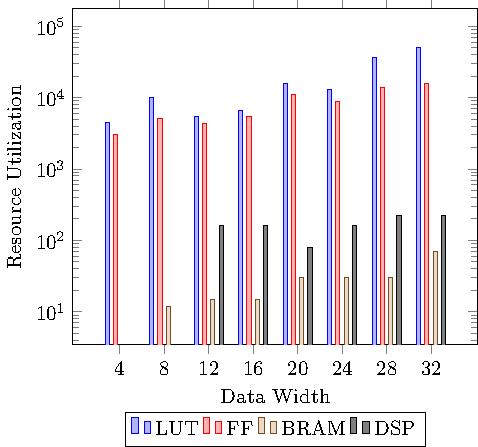
\includegraphics[width=0.65\columnwidth]{Figures/SigmoidResource.pdf}}
\subfigure[Resource utilization for ReLU Activation function]{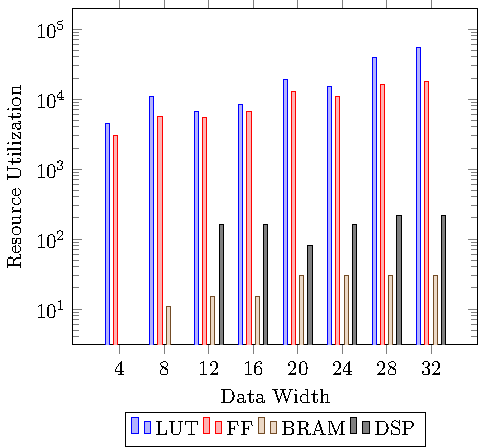
\includegraphics[width=0.65\columnwidth]{Figures/ReLUResource.pdf}}
\subfigure[Resource utilization for sigmoid Activation function with varying depth and datawidth 16]{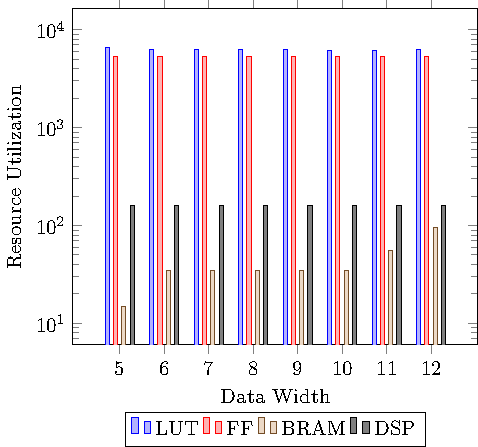
\includegraphics[width=0.65\columnwidth]{Figures/VarSigmoid16Width.pdf}}
\subfigure[Comparison of accuracy for Sigmoid and ReLU activation functions]
{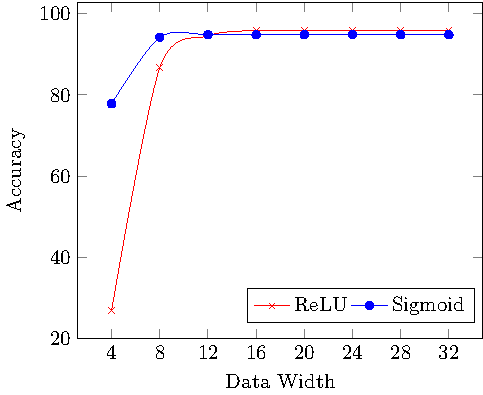
\includegraphics[width=0.62\columnwidth]{Figures/Accuracy.pdf}}
\subfigure[Detection accuracy and varying sigmoid memory depth]{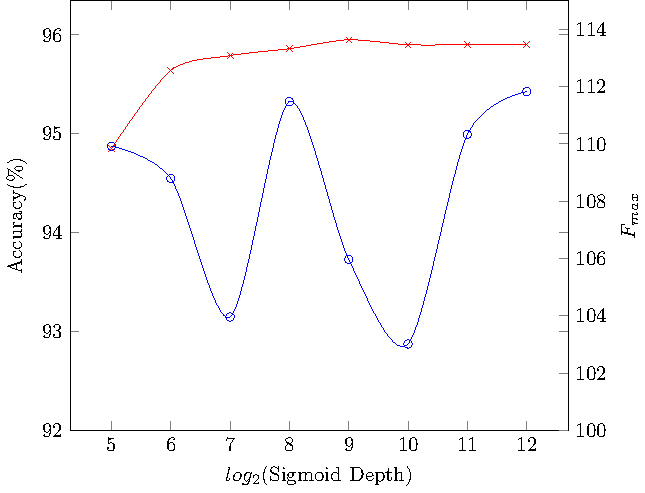
\includegraphics[width=0.65\columnwidth]{Figures/AccuracyVarSigmoid.pdf}}
\subfigure[Datawidth vs Maximum Frequency and Power consumption]{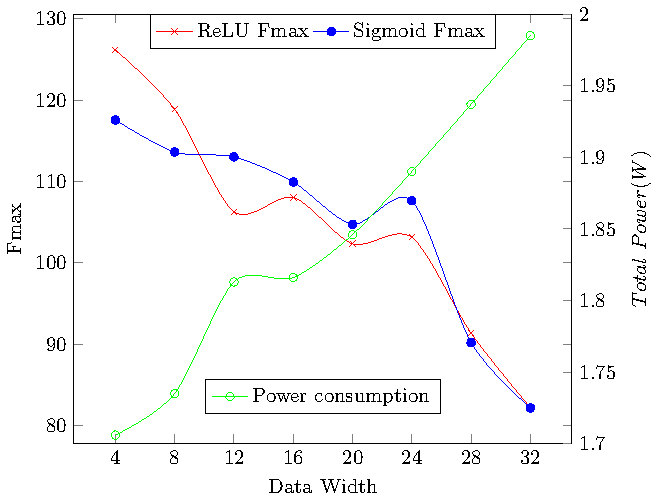
\includegraphics[width=0.65\columnwidth]{Figures/Timing.pdf}}
\caption{Evaluation results in terms of resource utilization, power consumption and maximum clock performance for different neural networks generated by ZyNet}
\end{figure*}

In this section we discuss the implementation results and performance of ZyNET based DNNs.
Multiple DNNs targeting the popular MNIST dataset is implemented and evaluated through both simulation and hardware validation.
The popular dataset for handwritten digit recognition uses 30000 images for training and 10000 images for testing.
The weights and biases for the network was initially determined through the corresponding software implementation and used for pre-training hardware implementation.
The software implementation with 30 epoch training provides 96.52\% detection accuracy for the testing set.

All implementations follow a 5 layer architecture with 784 neurons in input layer, 2 hidden layers with 30 neurons each and 1 hidden layer with 10 neurons and an output layer with 10 neurons.
The output layer is connected to a \emph{hardmax} module to detect the neuron with maximum output value.
All designs are simulated and implemented with Xilinx Vivado 2018.3 version and hardware validated on ZedBoard having an XC7Z020-CLG484 SoC and 512MB external DDR3 memory. 
All implementations use Vivado default settings and do not apply any optimization (timing,area or power). 

The DNN implementation was evaluated for both Sigmoid and ReLU activation functions for varying datawidth.
Fig.~\ref{fig:accuracy} shows the relation between the detection accuracy and datawidth.
It could be seen that for very small datawidth (such as 4 and 8 bits), Sigmoid-based function implementation outperforms ReLU-based implementation.
As the width increases, ReLU has slight advantage over Sigmoid implementation and accuracy of both implementations becomes constant beyond 12-bits.
Sigmoid implementation gives a maximum of 94.86\% detection accuracy and ReLU gives a maximum of 95.87\%.
The degradation in the result compared to software implementation can be attributed to the error introduced due to fixed point representation of weights, biases and input data.
Still the approximation causes less than 1\% error but gives considerable advantage in terms of resource utilization and clock performance.

Figures~5(a) and 5(b) compares the resource utilization of the DNNs for different data widths in terms of LUTs, flip-flops, Block RAMs and DSP slices while using the two different activation functions.
Since the RTL code generated by ZyNet does not explicitly instantiates any IP cores, for smaller designs the implementation tool (Vivado) automatically maps the multipliers and weight memory blocks into LUTs and flip-flops.
For larger data size, the lookup table used for implementing Sigmoid function are mapped to Block RAMs, which considerably increases the BRAM utilization.
For example, for 32-bit implementation, Sigmoid-based implementation requires 50350 LUTs, 15544 flip-flops, 70 BRAMs and 220 DSP slices.
At the same time ReLU-based implementation requires 54559 LUTs, 18074 flip-flops, 30 BRAMs and 220 DSP slices.
These numbers roughly maps to 94.6\% LUTs, 17\% flip-flops, 21.4\% BRAMs and 100\% DSP slices of xc7z020clg484-1 chip used in the Zed Board.
It should be noted that 16-bit implementation also consumes 220 DSP slices and as discussed before for larger networks the tool automatically maps the multipliers into LUTs and flip-flops.
Thus the largest network size is constrained by the number of LUTs available in the device. 

Another interesting result is the size of the Sigmoid look-up-table and the detection accuracy.
Fig.~5(e) shows the relation between the number of address bits used for Sigmoid LUT (sigmoid memory depth is $2^{address \_bits}$) and detection accuracy.
Here the datawidth is kept at a constant value of 16.
Experiments showed that the accuracy is quite low when the number of address bits is less than the sum of integer bits used to represent input values and weight values.
Here the minimum value is set as 5 bits, since the implementation uses 1-bit integer value for input and 4-bits for weight.
It could be seen that the Accuracy initially increases and remains constant after 8 bits.
Comparing it with Fig.~5(c), it could be seen that the resource utilization remain constant between LUT address width 6 to 10.
At the same time detection accuracy increases from 95.64\% to 95.95\% between these values.
The constant resource utilization is attributed the granularity of BRAM available in the device, which is 18Kb for 7-series Xilinx FPGAs.
Beyond 10-bits, resource utilization increases due to more BRAMs are required for implementing Sigmoid LUTs.
The detection accuracy also slightly reduces (95.90\%) remains constant.
The maximum clock frequency varies between 103~MHz and 111~MHz due to placement algorithm of the implementation tool.

Fig.~4(f) shows the maximum clock performance of the DNN for varying datawidth with two activation functions.
In most cases Sigmoid implementation outperforms ReLU implementation, but on Zynq platforms most of the other design components will be running at 100MHz, which is achieved by both implementations upto 24-bit wide implementations.
The plot also shows the power consumption of ZedBoard for Sigmoid-based network when running at 100 MHz clock frequency.
It varies between 1.706~W and 1.985~W depending on the datawidth (resource utilization).
Comparing it with the other popular edge device Raspberry-Pi3, the power consumption is in the range of 2.7W to 3.1W. 

Finally comparing the throughput, ZyNet based network on ZedBoard running at 100 MHz has a detection speed of 7.84 us/sample. On a Raspberry Pi3 platform using tensor flow, the throughput is 266 us/sample. On a standard computer with Intel i7 processor and 16GB RAM, the throughput for the same network is 30us/sample. This clearly demonstrates the advantage of reconfigurable platforms for edge devices in terms of throughput and power consumption.
\section{Conclusion and Future}
\label{sec_conclusion}
In this work we discussed the implementation of ZyNet, a Python package for automating deep neural network implementation on low-cost FPGA-based edge computing devices.
Results show that the implementation are capable of achieving high accuracy and clock performance with low resource utilization.
The proposed platform is capable of outperforming pure software implementation by more than 4$times$ on high-end machines and by several orders on other embedded platforms.

The main limitation of current release of ZyNet is that it supports only fully connected hidden layers.
In the future more varieties of networks will be supported on ZyNet such as CNNs and RNNs.
Other low-end platforms such as Intel Arria will be supported for automated system implementation.
The package is available in the public domain through the Python Package Index~(PyPI) repository and example designs are available through the git repository~\cite{zynetgit}. 

\bibliographystyle{IEEEtran}
\bibliography{fpt}
\end{document}
